%%%%%%%%%%%%%%%%%%%%%%%%%%%%%%%%%%%%%%%%%%%%%%%%%%%%%%%%%%%%%%%%%%%%%%%%%%%%%%%%
\section{Orbit Determination and Parameter Estimation}
%%%%%%%%%%%%%%%%%%%%%%%%%%%%%%%%%%%%%%%%%%%%%%%%%%%%%%%%%%%%%%%%%%%%%%%%%%%%%%%%

Predicting the state of a satellite given an initial condition, $\mathbf{x}_0$,
and models which constitute the equations of motion of the satellite,
$\dot{\mathbf{x}}=f(t,\mathbf{x})$, is a straightforward task involving the
solution of an initial value problem (IVP) in the form of an ordinary
differential equation (ODE). Furthermore, the accuracy of this solution can be
traded off against the computational expense of the prediction. However the
inverse problem  is more involved, that is, given a set of observations in the
dynamical system, we would like to estimate the trajectory of the satellite and
the parameters describing the dynamical models.

\begin{itemize}
    \item Orbit of asteroid
    \item Orbit of spacecraft
    \item Rotation of asteroid (rate + principle axes)
    \item Gravitational potential of asteroid
\end{itemize}

%%%%%%%%%%%%%%%%%%%%%%%%%%%%%%%%%%%%%%%%%%%%%%%%%%%%%%%%%%%%%%%%%%%%%%%%%%%%%%%%
\subsubsection{Weighted Least-Squares Estimation}
%%%%%%%%%%%%%%%%%%%%%%%%%%%%%%%%%%%%%%%%%%%%%%%%%%%%%%%%%%%%%%%%%%%%%%%%%%%%%%%%



\begin{equation}
    H=\frac{\partial{\mathbf{h}(x_0)}}{\partial{\mathbf{q}}}\bigg|_{\mathbf{x}_0}
\end{equation}

\begin{equation}
    \Delta{\mathbf{q}}=K(H^{T}W\Delta{\mathbf{h}})
\end{equation}

\begin{equation}
    K=(H^{T}WH)^{-1}
\end{equation}

\subsubsection{Linearization \& Normal Equations}

\subsubsection{Filtering}


 \noindent{}A CEKF consists of 3 main steps, namely: \textit{Initialisation (0)}, \textit{Prediction (1)} and \textit{Correction (2)}, where steps 1 \& 2 are iterated through $K-1$ times, where $K$ ($K\in\mathbb{Z}^+$) quantifies the number of Epochs.

 \begin{itemize}
     \item \textbf{Step (0) Initialisation}: The \textit{a posteriori} estimate of the initial state ($\hat{x}_0^+$) is determined according to the expectation of the true value $x_0$. The initial state error co-variance matrix is calculated according to the expectation of the co-variance between $\hat{x}_0^+$ and $x_0$. Within the context of satellite tracking, a predefined $\hat{x}_0^+$ will be used throughout the CEKF analysis to analyse the performance as a result of the selection of hyper-parameters: $\bm{Q}_{k-1}$ and $\bm{R}_k$.
     \item \textbf{Step (1) Prediction}: Project the state and its co-variance matrix at $k-1$ one step forward in order to obtain the \textit{a priori} estimates at $k$ according to the system dynamics. $\bm{Q}_{k-1}$ is implemented, then this contributes to the \textit{a priori} estimate of $P_k^{}$.
    \item \textbf{Step (2) Correction}: The measurements at $k$ are then compared with the predicted state according to system dynamics (\textit{a priori} estimate) providing the \textit{measurement innovation} ($\Delta{\rho}_k$). \textit{innovation co-variance} ($S_k$) and $H_k$ are then calculated and used to obtain the \textit{Kalman gain} ($\overline{K}_k$). Finally the \textit{a posteriori} estimate of the state ($\hat{x}_k^+$) and co-variance ($P_k^+$) are determined. $k$ is incremented by a step forward and the process from step 1 is repeated for all Epochs.
 \end{itemize}

\begin{figure}[htp]
    \centering
    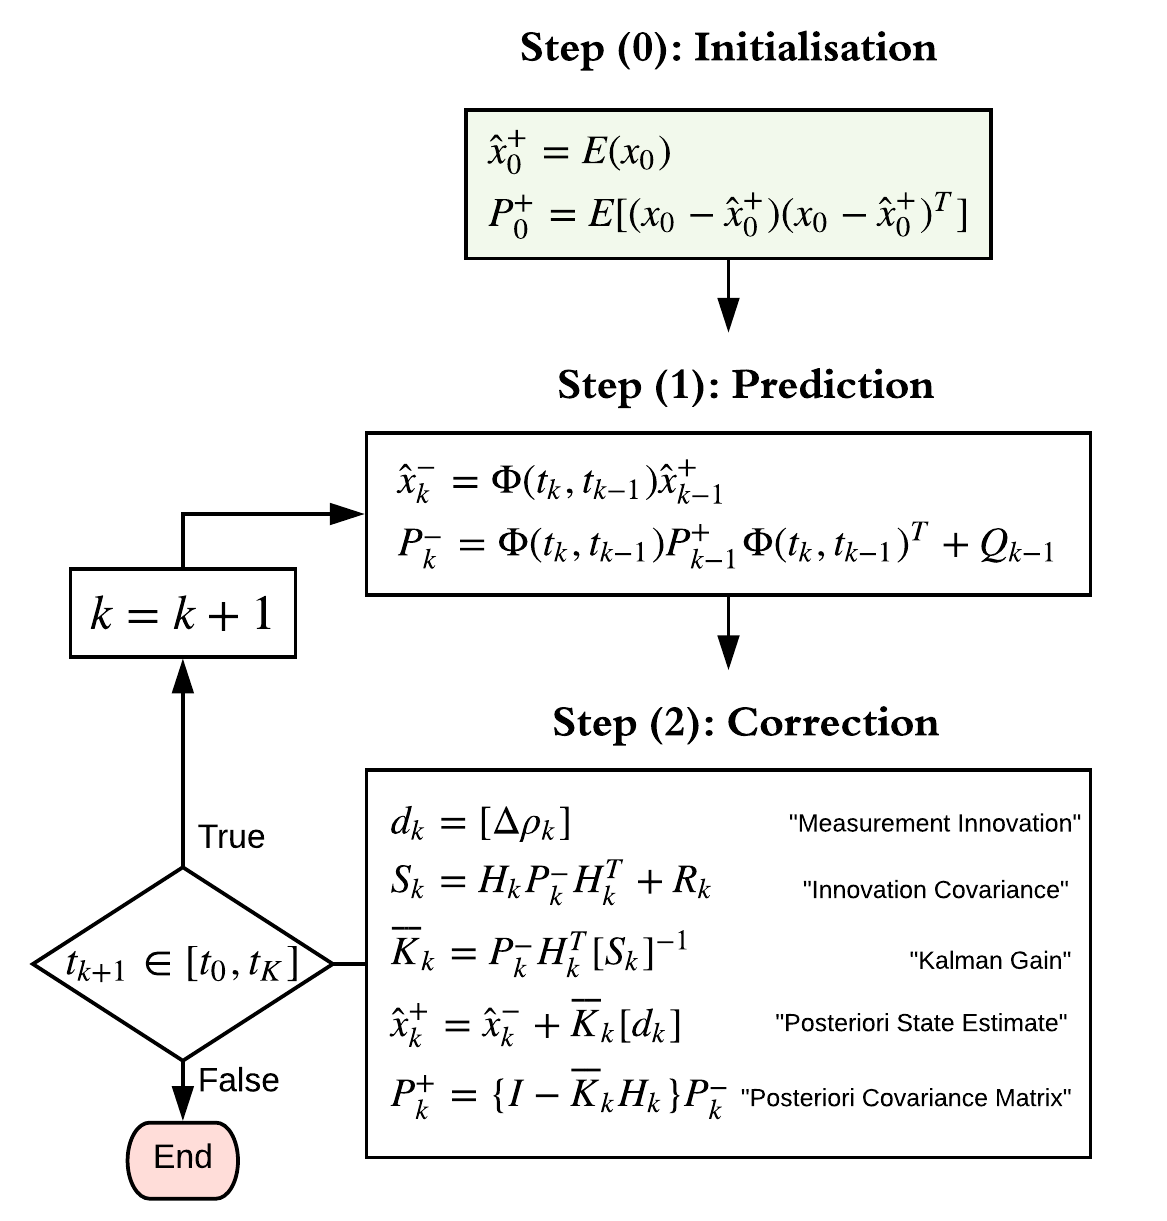
\includegraphics[width=0.55\linewidth]{graphics/CEKF.png}
    \caption{CEKF flow diagram for process of tracking and data prediction including all equations \cite{3}.}
    \label{fig:CEKF}
\end{figure}


\begin{figure}[htp]
    \centering
    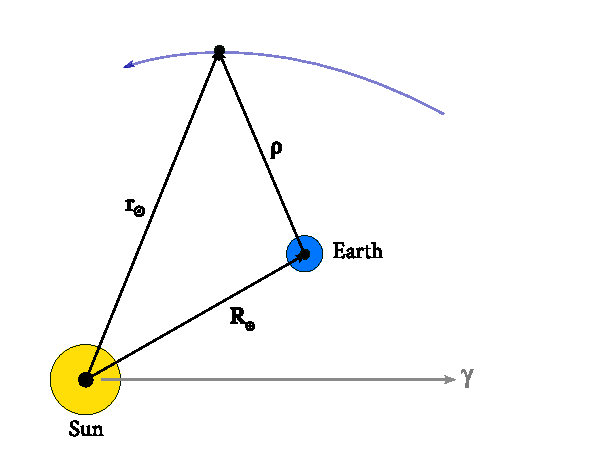
\includegraphics[width=0.5\linewidth]{graphics/pod-1.pdf}
    \caption{Orbit determination of asteroid using range observations from Earth ($\rho$).}
    \label{fig:my_label}
\end{figure}
